%%%% Proceedings format for most of ACM conferences (with the exceptions listed below) and all ICPS volumes.
%\documentclass[sigconf]{acmart}
%%%% As of March 2017, [siggraph] is no longer used. Please use sigconf (above) for SIGGRAPH conferences.

%%%% Proceedings format for SIGPLAN conferences 
% \documentclass[sigplan, anonymous, review]{acmart}

%%%% Proceedings format for SIGCHI conferences
\documentclass[sigchi]{acmart}

%%%% To use the SIGCHI extended abstract template, please visit
% https://www.overleaf.com/read/zzzfqvkmrfzn

\usepackage{booktabs} % For formal tables

% For accent characters
\usepackage[utf8]{inputenc}
\usepackage[T1]{fontenc}

% Copyright
\setcopyright{none}
%\setcopyright{acmcopyright}
%\setcopyright{acmlicensed}
%\setcopyright{rightsretained}
%\setcopyright{usgov}
%\setcopyright{usgovmixed}
%\setcopyright{cagov}
%\setcopyright{cagovmixed}


% DOI
%\acmDOI{10.475/123_4}

% ISBN
%\acmISBN{123-4567-24-567/08/06}

%Conference
%\acmConference[WOODSTOCK'97]{ACM Woodstock conference}{July 1997}{El Paso, Texas USA} 
%\acmYear{1997}
%\copyrightyear{2016}

%\acmPrice{15.00}


\begin{document}
\title{GANmons: Sketchable Monsters from Generative Adversarial Networks}
%\titlenote{Produces the permission block, and
%  copyright information}
\subtitle{CS 523 Project 3 Spring 2017}
\subtitlenote{Multimedia systems.
Generative models for creative intelligence. Prof. Angus Forbes.}


\author{Arthur Nishimoto}
%\authornote{Figured he'd be here 'cause he did a decent amount of the work.}
%\email{webmaster@marysville-ohio.com}

\author{Kristine Lee}
%\authornote{First because she wanted to take the lead on the paper and because she's awesome. But also liked the authors to be in alphabetical order by first name.}
%\orcid{1234-5678-9012}
%\affiliation{%
%  \institution{Institute for Clarity in Documentation}
%  \streetaddress{P.O. Box 1212}
%  \city{Dublin} 
%  \state{Ohio} 
%  \postcode{43017-6221}
%}
%\email{trovato@corporation.com}

\author{Xing Li}
%\authornote{Actually wrote code for this.}

% The default list of authors is too long for headers}
%\renewcommand{\shortauthors}{B. Trovato et al.}

\begin{abstract}
GANmon generates new images of monsters using Generative Adversarial Networks (GANs) trained on a dataset of existing creatures images scrapped from a database containing various Pokémon images. The goal is to train our neural network on a dataset of existing Pokémon images and attributes (name, type, abilities) to build the GANmon model, feed in sketches of new monsters, and return an image of the new GANmon consisting of attributes similar to the original Pokémon in the training set, but using the user’s sketch as the base input.
\end{abstract}

%\keywords{ACM proceedings, \LaTeX, text tagging}

%% Used in some conference proceedings e.g. sigplan and sigchi
\begin{teaserfigure}
   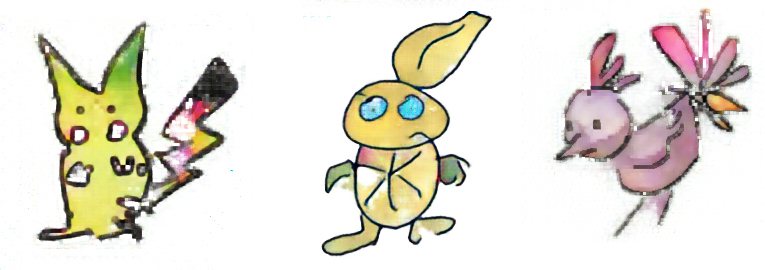
\includegraphics[width=6.8in]{figures/6A}
%   \caption{This is a teaser}
   \label{fig:teaser}
\end{teaserfigure}

\maketitle

\section{Introduction}
The motivation behind this project was work done by Janelle Shane who used a recurrent neural network (RNN) to randomly generate Pokémon names, abilities, and attributes based on a training set of existing Pokémon names and abilities. A blogger going by Iguanamouth used the output of the RNN to create illustrations of those Pokémon. Drawing on this work as inspiration, rather than just generating Pokémon names and abilities, we aim to generate new Pokémon using a neural network to automatically provide illustrations based on official artist renderings of existing Pokémon\footnote{Some of the images in this paper is artwork from a Pokémon game or derived from artwork owned by Nintendo/Creatures Inc./GAME FREAK inc. TM. No copyright or trademark infringement is intended by the authors of this paper.}.

Our neural network is based on Christopher Hesse's TensorFlow implementation of pix2pix by Isola et. al. \cite{pix2pix-tensorflow,pix2pix}

\section{Related Work}
The use of GANs to produce novel images is a growing field of interest. In particular, we were interested in the generation of images based on 1) semantic information and 2) sketch-based input.

\subsection{Translating semantic information to imagery}

In Learning What and Where to Draw by Reed et al. build off of the notion of using Generative Adversarial Networks (GANs) to synthesize real-world images based off of a text description or label \cite{whatWhereToDraw}. The authors believe by incorporating finer grained details of the image such as a specific body part, action, and location on the image, a GAN can create more realistic and complex scenes. The results we would like to accomplish with GANmons is similar to what Reed et al. accomplished, but beyond the scope of what we could accomplish at this time.

\subsection{Mapping sketches to images}

In the Sketchy paper, the authors discuss a few hurdles that arise when attempting to map human-input sketches to a desired output \cite{sketchy}. Human artists are imprecise: prone to exaggerating features or dropping information according to abstract semantic significance. The process described in this paper involved generating a dataset of hand-drawn renderings of images, and using classification to group images into different semantic categories.

An interesting dilemma regarding our own training data is that the images are already artistic renderings—if more professional than sketches produced by the average user. Many image-generating neural networks we researched are focused on creating “convincing”—often photorealistic—images. Unlike our own model, those GANs are trained on large sets of photographs. A few exceptions to this include an implementation of sketch-rnn \cite{2017arXiv170403477H} and Chainer-DCGAN \cite{chainer-DCGAN}.

Rather than specific pixel (raster) information, sketch-rnn utilizes a sequence-to-sequence framework of “motor actions” that represent the drawing of a stroke. While this implementation was perhaps more pertinent to the notion of cartoon-like renderings, we felt it would not be possible to generate sketch data for training in such a short span of time. However, generating a database of sketches was not inherent to the purposes of our project; Chainer-DCGAN follows a more traditional DCGAN implementation to generate manga-like images.

\section{Implementation}
This project consists of three main components: the web-scraper which was used to collect the images used as part of the training set, the TensorFlow application used to train, build , and test the model, and the web interface front-end used to allow the user to create or upload an image, which is then processed by the TensorFlow model, and then displays the result back to the user. The TensorFlow model was trained on the 18-node CAVE2 computing cluster at the Electronic Visualization Laboratory at the University of Illinois at Chicago \cite{CAVE2_2013}. While we were developing a version of pix2pix-tensorflow that would run distributively across the cluster, the early training was done on a single node with an nVidia 1070 GPU.

\subsection{Training Set}

\begin{figure}[h]
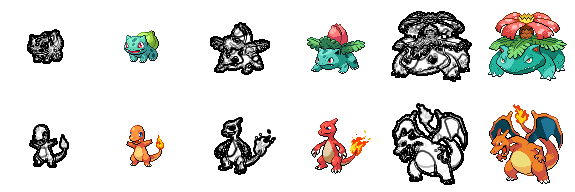
\includegraphics[width=3.25in]{figures/ModelA-TrainingPairs.jpg}
\caption{Example ModelA Training Pairs.}
\end{figure}

The images used to train our TensorFlow model consisted of two types: sprites and artist renderings. The web-scraper pulls images from the Bulbapedia image archive. For the initial training set ‘ModelA', 649 images of the front and back colored sprites from generation 5 games was trained for 500 epochs for ~8 hours. Validation tests used sketches, artist renderings, and the remaining generation 5 sprites not used in the training set. Our model follows the original pix2pix consisting of side-by-side image pairs. The line edge input is on the left and the desired output is on the right.

\begin{figure}[h]
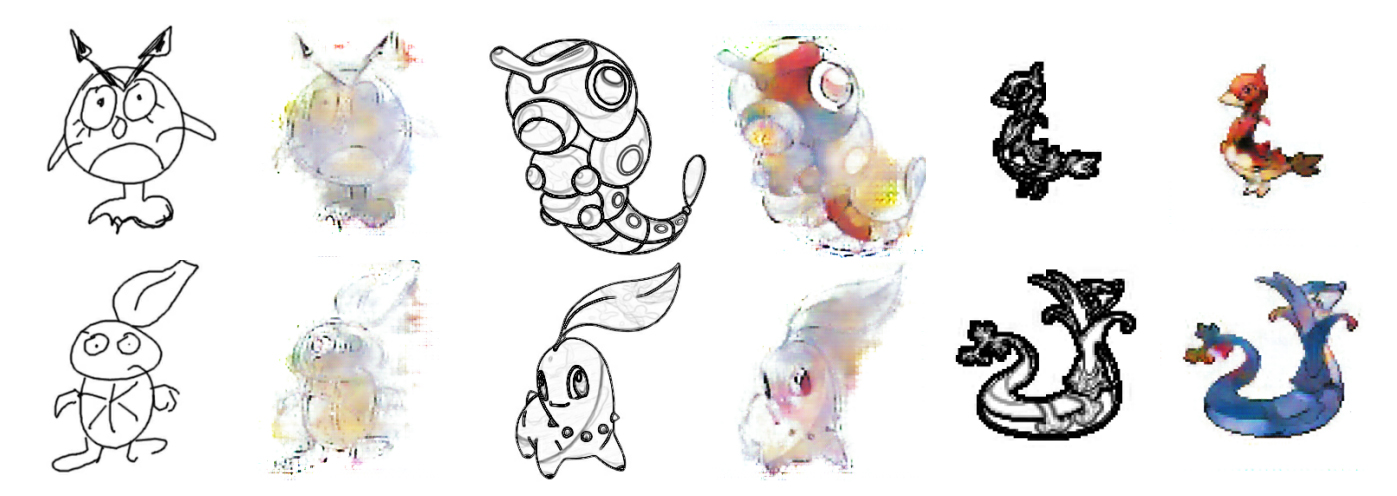
\includegraphics[width=3.25in]{figures/ModelA-Valid-649sprite-500epoch.jpg}
\caption{Example ModelA Validation Test Images. For each image pair the input is on the left, model output on the right.}
\end{figure}

Based on our initial validation tests, we introduced 3 different line weighted images to the test set. These were generated using the ‘Find Edges’ filter in Photoshop. This revised version of ModelA was trained using 9846 total sprites from generation 2-5 games with the 3 line weights variants per sprite. This was trained for 200 epochs over 61 hours. While this was training, ModelB was training on a different CAVE2 node. The input test sketches were processed with an image filter to more closely match the pixelated training images.

\begin{figure}[h]
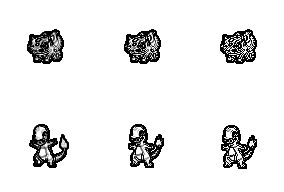
\includegraphics[width=3.25in]{figures/ModelA-LineWeights.jpg}
\caption{Revised ModelA Line Weights.}
\end{figure}


\begin{figure}[h]
\includegraphics[width=3.25in]{figures/Abra2-Edges.jpg}
\caption{Example ModelB (Top) and ModelB1 (Bottom) Training Pairs.}
\end{figure}


ModelB images uses the artist renderings of the 151 Pokémon from generation 1. Each Pokémon has 6 to 12 different images. The same edge filter used in ModelA was used, but due to the variable, but higher resolution of these renders compared to the 256 by 256 sprites, the edge filter yielded clearer results which could be used to match the input sketches.

\begin{figure}[h]
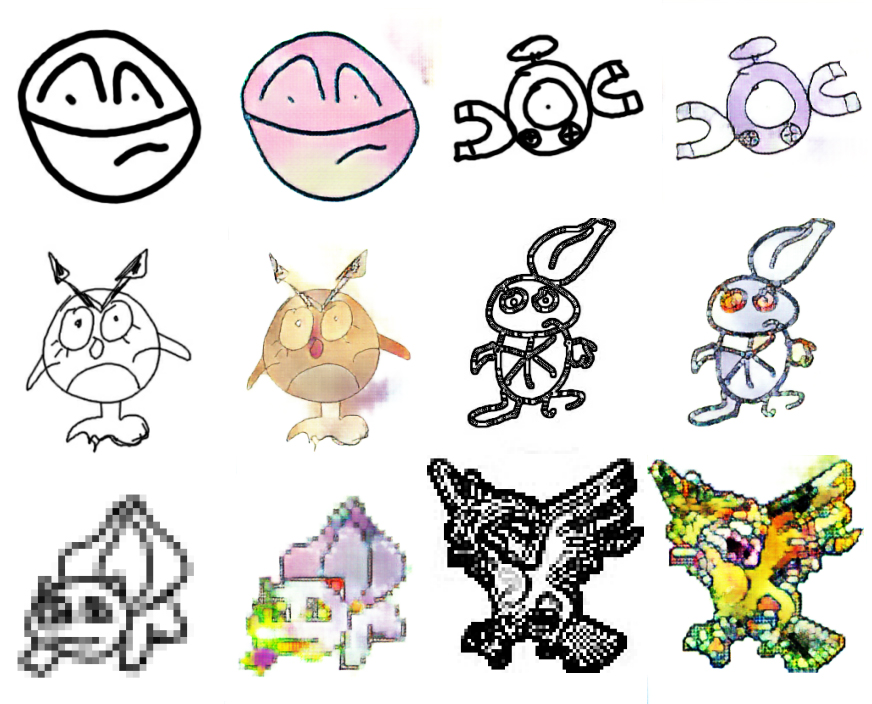
\includegraphics[width=3.25in]{figures/ModelB-Valid-1200render-70epoch.jpg}
\caption{ModelB Results over 1200 epochs.}
\end{figure}

ModelA1 uses a threshold filter to generate the line render instead of the edge filter used in ModelA. This model was trained using 3952 generation 2 through 5 front sprites and trained for 200 epochs over 18 hours.

ModelB1 also uses the same threshold filter as ModelA1, but with the artist renderings. Models A2 and B2 are continuations of the A1 and B1 models trained for a longer period of time. Due to the larger training set in A2 versus B2, in the same amount of time B2 progressed to over 1700 epochs while A2 is at 800.

\subsection{pix2pix}
The generative adversarial neural network used in the generation of the images was proposed in the paper Image-to-Image Translation with Conditional Adversarial Networks. The consists of a generator and a discriminator both in the form convolution-BatchNorm-ReLu. In addition they add skip connections in the generator to avoid bottlenecks due to the amount of low level information shared by both the input and output. Due to the fact that simple L2 or L1 loss results in blurry images, the descriminator architecture only penalizes structure at the scale of patches where it determines whether a N by N patch in the image is fake or real. Due the fact that the descriminator can run on patch sizes that are much smaller than the image itself, runtime is drastically improved. 

\subsection{Cluster}
In our attempted to distribute load to across several Lyra nodes, we looked into dividing up the code so that it could be run in parallel. However, we ran into networking issues where the main Lyra node was unable to detect its workers threads even though the worker and main threads were running on each of the clusters.

\subsection{Web Interface}

\begin{figure*}
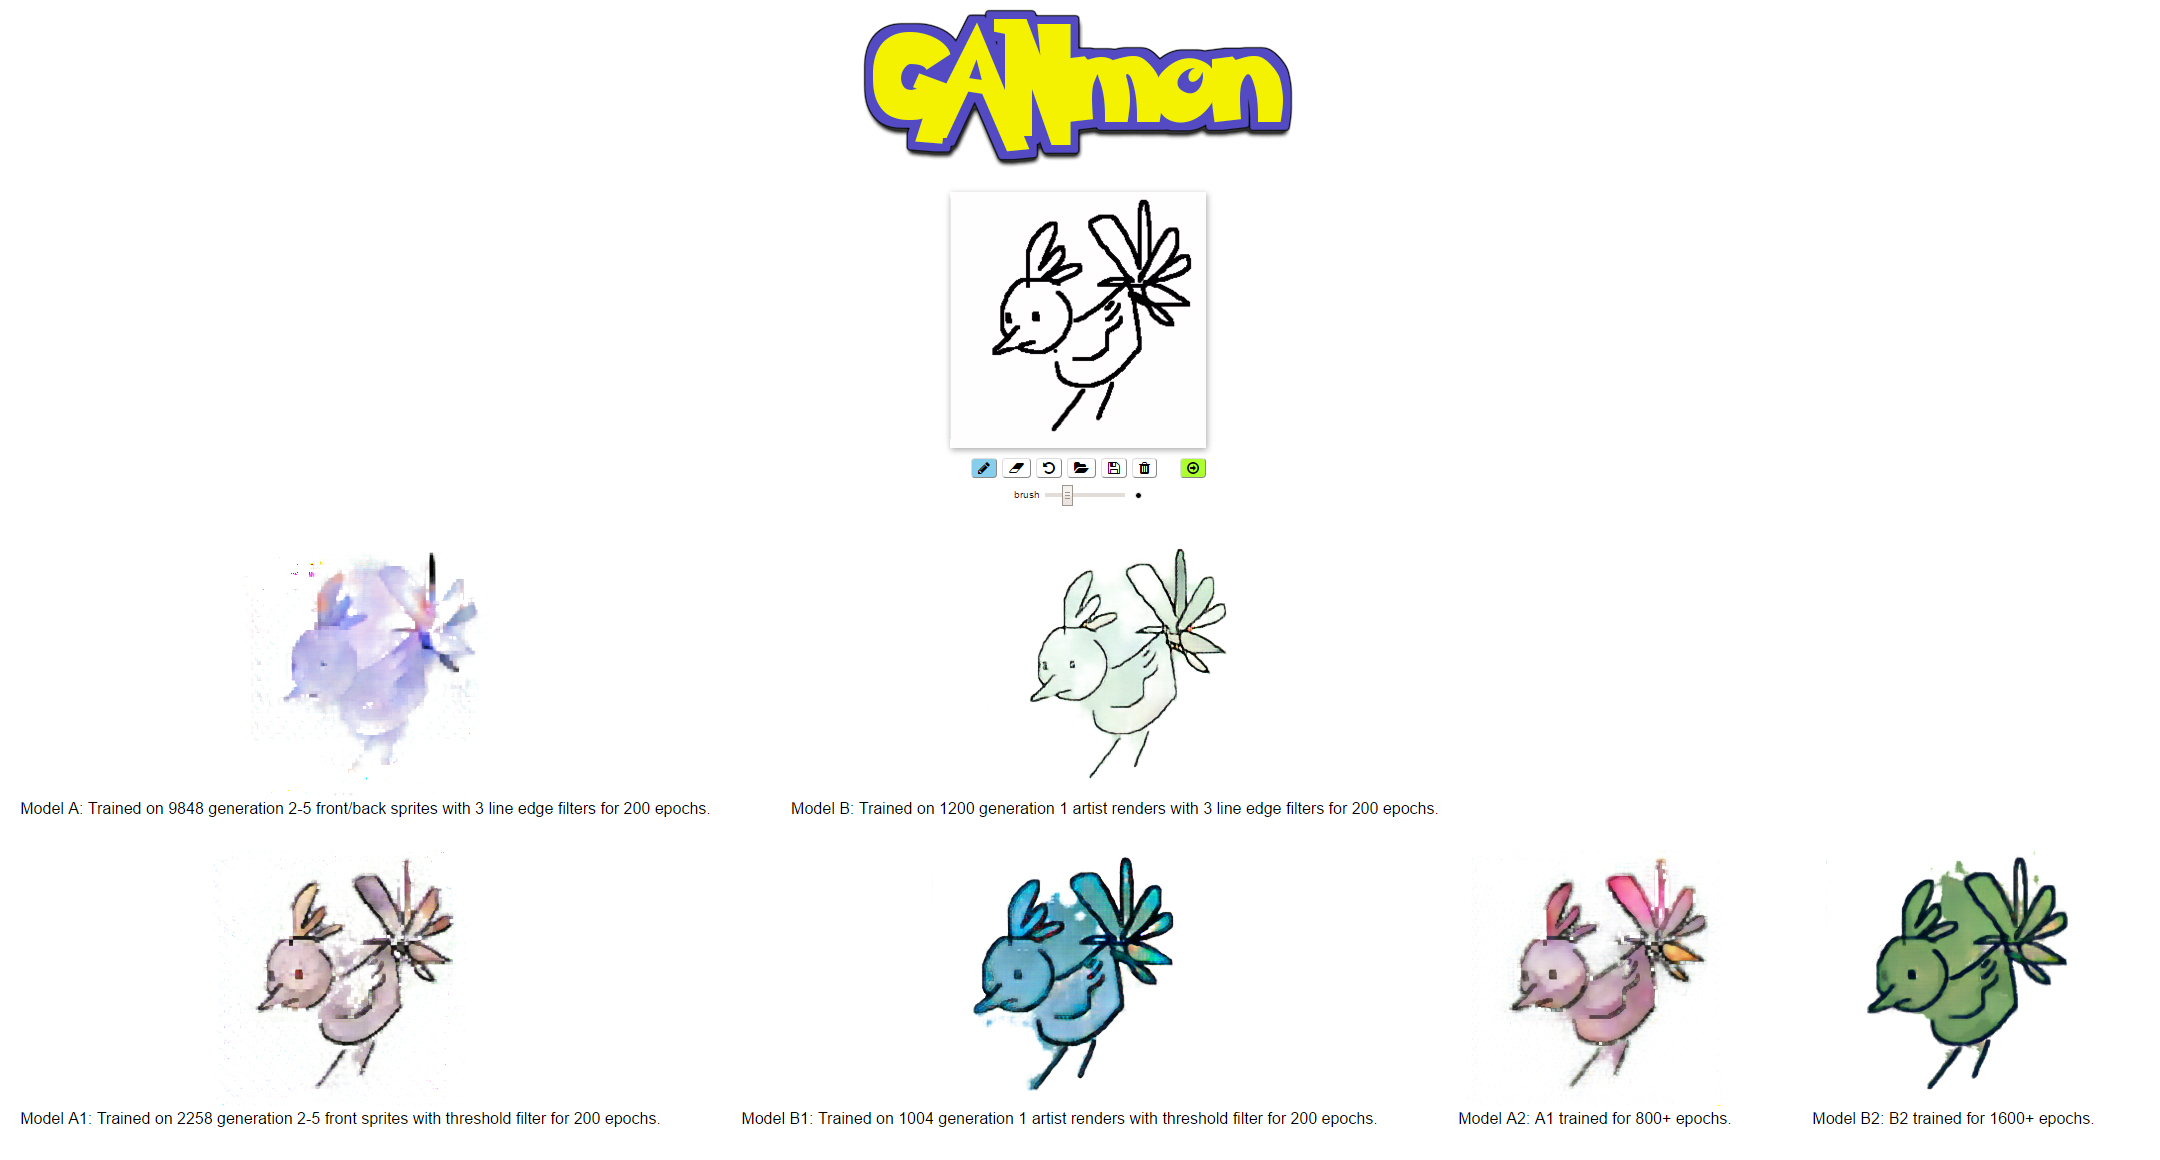
\includegraphics[width=7in]{figures/GANmonWeb.jpg}
\caption{GANmon Web Interface.}
\end{figure*}

We provided a web interface using HTML5 canvas to allow users to explore the capabilities of the GANmon generator. The user may draw a 256-by-256-pixel black-and-white image onto the canvas, or upload an existing image for processing.

During the processing phase a bash script on the server runs our TensorFlow application on the input image. As our TensorFlow application runs on the GPU, each of the 6 models are run on a different node using ssh. Once the last process is done, the model results are returned to the user and displayed next to each other on the web page for comparison purposes.

Because of the art style the neural network was trained on, small changes to the lines of the input could potentially produce dramatic differences in output.

\begin{figure}[h]
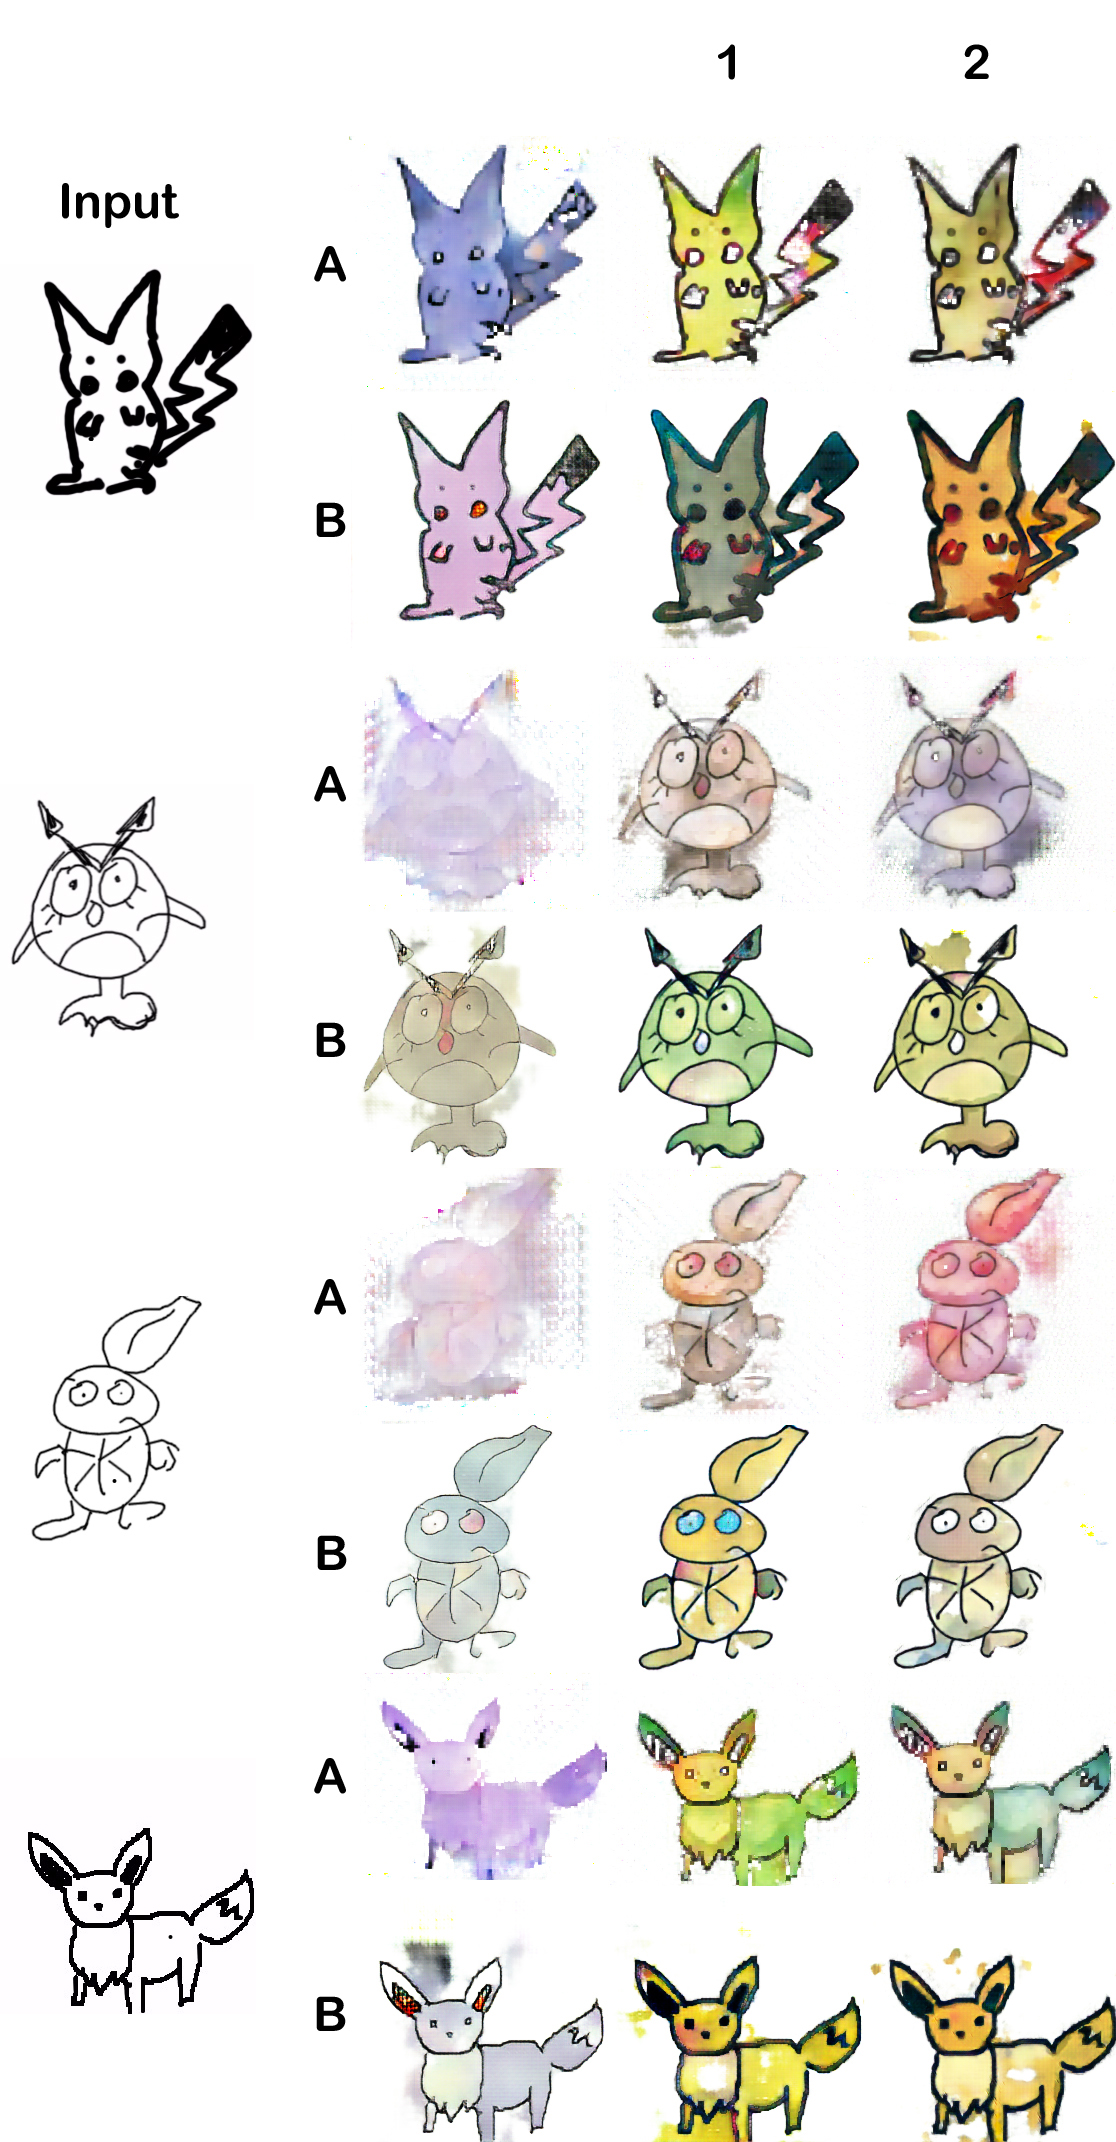
\includegraphics[width=4in]{figures/FinalResultsSmall.jpg}
\caption{Results for all models: Sprites (A), Artist Renders (B), Edge Filter (1), and Threshold Filter(2).}
\end{figure}

\section{Conclusion}


In this paper, we used a generative adversarial network to generate images of 'GANmons' from a trained model of Pokémon and an input sketch. In our exploration of this technique we utilized multiple types of images for training and developed an interactive web interface for drawing a sketch and processing that input on the models. Our iterative approach explored both using the original game sprites (ModelA) and artist renderings (ModelB) with an line edge filter (A1, B1) and a threshold filter (A2, B2). Depending on the style and quality of the input, the resulting image can have varying results. For example in figure 7, some images yielded better results using the line edge filter while others were better with the threshold filter. Similarly some inputs worked better with the sprite model versus the artist renders and vice versa. Future work could improve the quality of the results though longer training of the model as well as labeling of features in the training sets.

\bibliographystyle{ACM-Reference-Format}
\bibliography{references} 
\end{document}
